\section{}
A crane 100 m tall is loading a container full of feathers and delicate glass figurines weighing 5 metric tons onto a cargo ship. While the container is in the air, there is an emergency shutdown of the crane and the case is left hanging for a short time. During this time, winds cause the arm of the crane to vibrate vertically at a frequency of 4 Hz with an amplitude of 5 cm. The supporting cable has an effective stiffness of $k = \frac{100}{L}$ MN/m, where $L$ is the length of exposed cable in metres (neglect changes in $L$ due to vibration).

\begin{figure}[h]
\centering
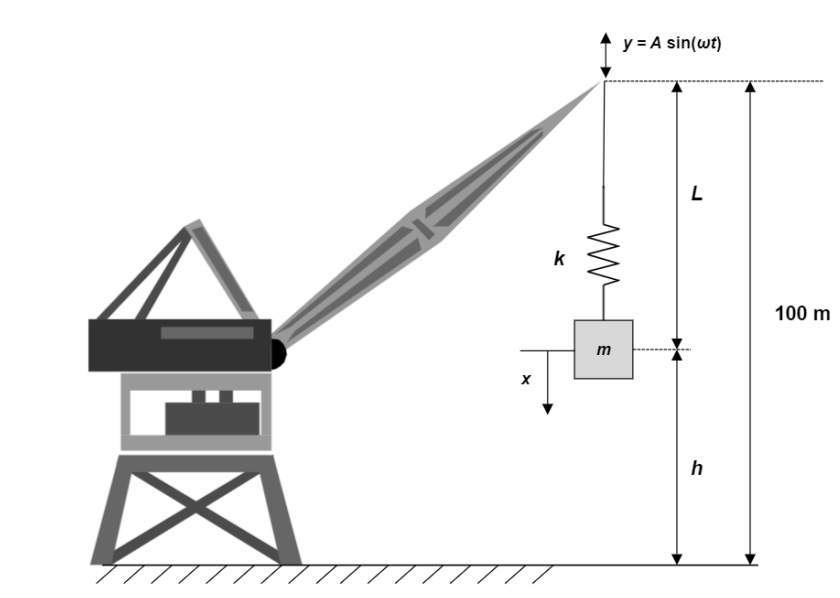
\includegraphics[width=0.5\textwidth]{Questions/Figures/q2 problem diagram.png}
\end{figure}
\FloatBarrier
\begin{enumerate}[label=(\alph*)]
    \item (2 pts) Determine the cable length $L$ at which the transmissibility would be exactly 1.
    \item (5 pts) Assuming steady state vibration, determine all possible heights $h$ at which the crate would hit the ground.
    \item (3 pts) After the emergency is dealt with, operations resume as the wind continues to excite the crane arm. The crane needs to lift shipments 80 m high to place it onto the cargo ships. What is the smallest mass of cargo that can be lifted in these conditions without shaking with an amplitude greater than 4 cm? Assume $\omega > p$.
\end{enumerate}
\FloatBarrier
\subsection*{Solution}
\subsection{}
First, we must choose the proper model for the system. A simple undamped spring-mass with base excitation model is appropriate. Assume the weight of the cable is negligible. 

The transmissibility is then
\begin{align*}
    \text{TR} &= \frac{\left(\frac{\omega}{p}\right)^2}{1 - \left(\frac{\omega}{p}\right)^2} \\
\end{align*}
converting $f = 4$ Hz to $\omega = 2\pi f = 8\pi$ rad/sec, we can solve for $p$ when $\text{TR} = 1$
\begin{align*}
    1 &= \frac{\left(\frac{8\pi}{p}\right)^2}{1 - \left(\frac{8\pi}{p}\right)^2} \\
    1 - \left(\frac{8\pi}{p}\right)^2 &= \left(\frac{8\pi}{p}\right)^2 \\
    1 &= 2\left(\frac{8\pi}{p}\right)^2 \\
    \implies p &= 8\sqrt{2} \pi
\end{align*}
Since $p$ is defined as 
\begin{align*}
    p &= \sqrt{\frac{k}{m}}\\
    \implies k &= p^2m = (8\sqrt{2}\pi)^2 (5 \times 10^3) = 0.64\pi^2 \times 10^6 \text{ N/m} = 0.64\pi^2 \text{ MN/m}
\end{align*}
and since $k = \frac{100}{L}$, we can solve for $L$,
\begin{align*}
    \Aboxed{L &= \frac{100}{k} = \frac{100}{0.64\pi^2} = 15.8 \text{ m}}
\end{align*}

\subsection{}
The steady state vibration of the system is given by
\begin{align*}
    x(t) = A\left(\frac{1}{1 - \left(\frac{\omega}{p}\right)^2}\right)\sin(\omega t)
\end{align*}
where $x$ is the distance from the equilibrium position, $A$ is the amplitude, $\omega$ is the angular frequency of the excitation. Then, the amplitude is 
\begin{align*}
    X &= A \left(\frac{1}{1 - \left(\frac{\omega}{p}\right)^2}\right) \\
    &= 0.05 \left(\frac{1}{1 - \left(\frac{8\pi}{8\sqrt{2}\pi}\right)^2}\right) \\
    &= 0.1 \text{ m}
\end{align*}